\documentclass[border=10pt]{standalone}
\usepackage{tikz}
\usepackage[utf8]{inputenc}
\usepackage[T1]{fontenc}
\usetikzlibrary{patterns,arrows.meta}

\begin{document}

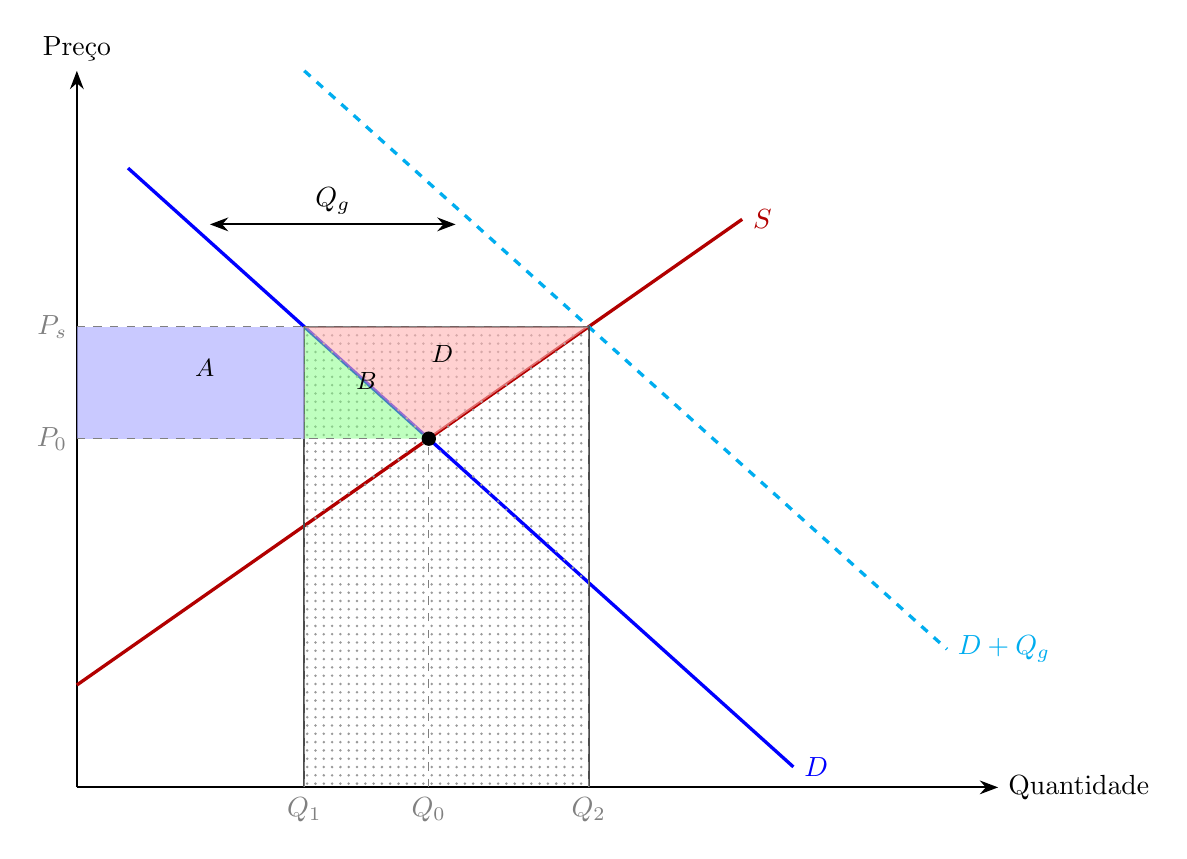
\begin{tikzpicture}[scale=1.3, >=Stealth]
    
    % Eixos
    \draw[thick,->] (0,0) -- (9,0) node[right] {Quantidade};
    \draw[thick,->] (0,0) -- (0,7) node[above] {Preço};
    
    % Curvas de oferta e demanda - mesmas da figura-9-11
    \draw[blue, very thick, domain=0.5:7] plot (\x, {6.5 - 0.9*\x}) node[right] {$D$};
    \draw[red!70!black, very thick, domain=0:6.5] plot (\x, {1.0 + 0.7*\x}) node[right] {$S$};
    
    % Pontos de equilíbrio
    % Equilíbrio original: interseção de D e S
    % 6.5 - 0.9*x = 1.0 + 0.7*x => 5.5 = 1.6*x => x = 3.4375, y = 3.406
    \coordinate (E0) at (3.4375, 3.406);  % Equilíbrio original
    \coordinate (Ps) at (0, 4.5);    % Preço sustentado
    
    % Coordenadas importantes
    % Q1: D em Ps=4.5: 4.5 = 6.5 - 0.9*x => x = 2.222
    % Q2: S em Ps=4.5: 4.5 = 1.0 + 0.7*x => x = 5.0
    \def\Qd{2.222}
    \def\Qeq{3.4375}
    \def\Qs{5.0}
    \def\Peq{3.406}
    \def\Ps{4.5}
    
    % Curva de demanda deslocada (tracejada) - deve cruzar S em (Q2, Ps) = (5.0, 4.5)
    % D+Qg deve passar por (5.0, 4.5) com inclinação -0.9
    % 4.5 = a - 0.9*5.0 => a = 4.5 + 4.5 = 9.0
    % Limitar para não exceder y=7: 7 = 9.0 - 0.9*x => x = 2.222
    \draw[cyan, very thick, dashed, domain=2.222:8.5] plot (\x, {9.0 - 0.9*\x}) node[right] {$D + Q_g$};
    
    % Retângulo pontilhado (custo do governo) - abaixo de Ps, entre Q1 e Q2
    \fill[pattern=dots, pattern color=black!40] (\Qd,0) rectangle (\Qs,\Ps);
    
    % Destacar as bordas do retângulo pontilhado
    \draw[thick, black!70] (\Qd,0) -- (\Qd,\Ps) -- (\Qs,\Ps) -- (\Qs,0);
    
    % Área A (excedente consumidor perdido)
    \fill[blue!30, opacity=0.7] (0,\Ps) -- (\Qd,\Ps) -- (\Qd,\Peq) -- (0,\Peq) -- cycle;
    
    % Área B (transferência/deadweight)
    \fill[green!50, opacity=0.5] (\Qd,\Ps) -- (\Qeq,\Peq) -- (\Qd,\Peq) -- cycle;
    
    % Área D (ganho produtor + deadweight) - triângulo acima de D e S, abaixo de Ps
    % Vértices: (Q0, P0), (Q2, Ps), (Q1, Ps)
    % Mas precisa seguir as curvas D e S
    % Pontos: onde D cruza linha horizontal Ps, onde S cruza linha horizontal Ps, e ponto de equilíbrio
    % D em Ps=4.5: 4.5 = 6.5 - 0.8*x => x = 2.5 (Q1)
    % S em Ps=4.5: 4.5 = 1.25 + 0.7*x => x = 4.64 ≈ 4.7 (Q2)
    % Triângulo: (2.5, 4.5), (4.7, 4.5), (3.5, 3.7)
    \fill[red!30, opacity=0.6] (\Qd,\Ps) -- (\Qs,\Ps) -- (\Qeq,\Peq) -- cycle;
    
    % Linhas tracejadas horizontais
    \draw[dashed, gray] (0,\Ps) node[left] {$P_s$} -- (\Qs,\Ps);
    \draw[dashed, gray] (0,\Peq) node[left] {$P_0$} -- (\Qeq,\Peq);
    
    % Linhas tracejadas verticais
    \draw[dashed, gray] (\Qd,0) node[below] {$Q_1$} -- (\Qd,\Ps);
    \draw[dashed, gray] (\Qeq,0) node[below] {$Q_0$} -- (\Qeq,\Peq);
    \draw[dashed, gray] (\Qs,0) node[below] {$Q_2$} -- (\Qs,\Ps);
    
    % Rótulos das áreas
    % Área A: retângulo (0, 3.7) a (2.5, 4.5) - centro: (1.25, 4.1)
    \node at (1.25, 4.1) {\small $A$};
    % Área B: triângulo (2.5, 4.5), (3.5, 3.7), (2.5, 3.7) - centro: (2.83, 3.97)
    \node at (2.83, 3.97) {\small $B$};
    % Área D: triângulo (2.5, 4.5), (4.7, 4.5), (3.5, 3.7) - centro: (3.57, 4.23)
    \node at (3.57, 4.23) {\small $D$};
    
    % Seta mostrando Qg - horizontal com setas nas duas extremidades
    % Escolher uma altura para mostrar a diferença, por exemplo y=5.5
    % D em y=5.5: 5.5 = 6.5 - 0.9*x => x = 1.111
    % D+Qg em y=5.5: 5.5 = 9.0 - 0.9*x => x = 3.889
    % Reduzir levemente o comprimento para não tocar as curvas
    \draw[<->, thick, black] (1.3, 5.5) -- (3.7, 5.5);
    \node[above] at (2.5, 5.5) {$Q_g$};
    
    % Pontos de equilíbrio
    \fill (E0) circle (2pt);
    
\end{tikzpicture}

\end{document}
